%% bare_conf.tex
%% V1.4b
%% 2015/08/26
%% by Michael Shell
%% See:
%% http://www.michaelshell.org/
%% for current contact information.
%%
%% This is a skeleton file demonstrating the use of IEEEtran.cls
%% (requires IEEEtran.cls version 1.8b or later) with an IEEE
%% conference paper.
%%
%% Support sites:
%% http://www.michaelshell.org/tex/ieeetran/
%% http://www.ctan.org/pkg/ieeetran
%% and
%% http://www.ieee.org/

%%*************************************************************************
%% Legal Notice:
%% This code is offered as-is without any warranty either expressed or
%% implied; without even the implied warranty of MERCHANTABILITY or
%% FITNESS FOR A PARTICULAR PURPOSE! 
%% User assumes all risk.
%% In no event shall the IEEE or any contributor to this code be liable for
%% any damages or losses, including, but not limited to, incidental,
%% consequential, or any other damages, resulting from the use or misuse
%% of any information contained here.
%%
%% All comments are the opinions of their respective authors and are not
%% necessarily endorsed by the IEEE.
%%
%% This work is distributed under the LaTeX Project Public License (LPPL)
%% ( http://www.latex-project.org/ ) version 1.3, and may be freely used,
%% distributed and modified. A copy of the LPPL, version 1.3, is included
%% in the base LaTeX documentation of all distributions of LaTeX released
%% 2003/12/01 or later.
%% Retain all contribution notices and credits.
%% ** Modified files should be clearly indicated as such, including  **
%% ** renaming them and changing author support contact information. **
%%*************************************************************************


% *** Authors should verify (and, if needed, correct) their LaTeX system  ***
% *** with the testflow diagnostic prior to trusting their LaTeX platform ***
% *** with production work. The IEEE's font choices and paper sizes can   ***
% *** trigger bugs that do not appear when using other class files.       ***                          ***
% The testflow support page is at:
% http://www.michaelshell.org/tex/testflow/



\documentclass[conference]{IEEEtran}
\usepackage{url}
\usepackage{graphicx}
\graphicspath{ {images/} }

\usepackage{listings}
\usepackage{color}

\definecolor{dkgreen}{rgb}{0,0.6,0}
\definecolor{gray}{rgb}{0.5,0.5,0.5}
\definecolor{mauve}{rgb}{0.58,0,0.82}

\lstset{frame=tb,
  language=Java,
  aboveskip=3mm,
  belowskip=3mm,
  showstringspaces=false,
  columns=flexible,
  basicstyle={\small\ttfamily},
  numbers=none,
  numberstyle=\tiny\color{gray},
  keywordstyle=\color{blue},
  commentstyle=\color{dkgreen},
  stringstyle=\color{mauve},
  breaklines=true,
  breakatwhitespace=true,
  tabsize=3
}

%
\ifCLASSINFOpdf
  % \usepackage[pdftex]{graphicx}
  % declare the path(s) where your graphic files are
  % \graphicspath{{../pdf/}{../jpeg/}}
  % and their extensions so you won't have to specify these with
  % every instance of \includegraphics
  % \DeclareGraphicsExtensions{.pdf,.jpeg,.png}
\else
  % or other class option (dvipsone, dvipdf, if not using dvips). graphicx
  % will default to the driver specified in the system graphics.cfg if no
  % driver is specified.
  % \usepackage[dvips]{graphicx}
  % declare the path(s) where your graphic files are
  % \graphicspath{{../eps/}}
  % and their extensions so you won't have to specify these with
  % every instance of \includegraphics
  % \DeclareGraphicsExtensions{.eps}
\fi



% correct bad hyphenation here
\hyphenation{op-tical net-works semi-conduc-tor}


\begin{document}

\title{Automatic Espresso Machine}

% author names and affiliations
% use a multiple column layout for up to three different
% affiliations
\author{\url{https://pabstaaron.github.io/AutoCoffeeMaker/} \\ \\ Aaron~Pabst, Ben~Nagel, Nathan~Donaldson}



% conference papers do not typically use \thanks and this command
% is locked out in conference mode. If really needed, such as for
% the acknowledgment of grants, issue a \IEEEoverridecommandlockouts
% after \documentclass

% for over three affiliations, or if they all won't fit within the width
% of the page, use this alternative format:
% 
%\author{\IEEEauthorblockN{Michael Shell\IEEEauthorrefmark{1},
%Homer Simpson\IEEEauthorrefmark{2},
%James Kirk\IEEEauthorrefmark{3}, 
%Montgomery Scott\IEEEauthorrefmark{3} and
%Eldon Tyrell\IEEEauthorrefmark{4}}
%\IEEEauthorblockA{\IEEEauthorrefmark{1}School of Electrical and Computer Engineering\\
%Georgia Institute of Technology,
%Atlanta, Georgia 30332--0250\\ Email: see http://www.michaelshell.org/contact.html}
%\IEEEauthorblockA{\IEEEauthorrefmark{2}Twentieth Century Fox, Springfield, USA\\
%Email: homer@thesimpsons.com}
%\IEEEauthorblockA{\IEEEauthorrefmark{3}Starfleet Academy, San Francisco, California 96678-2391\\
%Telephone: (800) 555--1212, Fax: (888) 555--1212}
%\IEEEauthorblockA{\IEEEauthorrefmark{4}Tyrell Inc., 123 Replicant Street, Los Angeles, California 90210--4321}}


% make the title area
\maketitle
% As a general rule, do not put math, special symbols or citations
% in the abstract
\begin{abstract}
% Imagine having a machine that would allow you to make the perfect cup of coffee
% right in your own home or office, without ever having to trek to the coffee
% shop. A machine that allows you to specify exactly how you like your coffee
% with exacting detail and optional scheduling at which point it will flawlessly
% produce that beverage for you. A machine that can recommend new beverages based
% on your and other users past preferences.
% 
% There are plenty of machines on the market that claim to be fully automatic,
% but none are capable of going all the way from raw ingredients to a finished
% beverage without any intervention from the user. With these
% machines, the user still has to manually froth milk, dispense flavoring
% syrup, and mix the beverage themselves; the machine only handles the grinding,
% tamping, and brewing tasks.
% These machines also provide a very limited scope of control to the user, giving them
% only a few options for dictating how they would like their coffee to be
% produced.
% Finally, most of these machines have very limited user interfaces and few have
% an option for remote control from a more user friendly device, such as a
% smart phone or tablet.
% 
% Our product differs by focusing on automation, personalization, and
% user-friendliness above all else. Our machine will house all ingredients
% internally, receive instructions wirelessly, and will have an automatic
% cleaning mechanism. The minimization of human interaction allows us to have
% complete control of the brewing and mixing process, allowing us to make a
% consistent cup of coffee. This also allows us to operate the machine
% wirelessly, allowing for streamlined UI capabilities and scheduled events.
% Autonomous control allows you to monitor the machine’s use, personal
% consumption habits, and ingredient consumption, while also giving the user the
% ability to tweak individual settings to make a personalized and reproducible
% cup of coffee. The machine itself will consist of a series of boilers,
% chillers, and pumps as well as a specially designed chamber for automatically
% frothing milk. These components will be driven from custom heater and chiller
% control circuitry as well as an embedded Linux controller. The physical device
% will be backed by some remote user-interface and a database for storing
% ingredient information and user data.

Making espresso is difficult. It takes several pieces of bulky equipment and a
lot of practice to consistently get right. However, most of the difficult tasks
involved in the espresso making process can be automated in a way that is predictable and
consistent. There are several machines on the market that do successfully
automate the process, but none of these machines make espresso in the same way that
skilled baristas do and the quality of the output reflects this. By creating a
machine that mimics a human barista, these automatic espresso machines can be
superseded.
\end{abstract}


% What is the project motivation? 
%
% TODO - Could use a citation or two in here
% TODO - Add more background information
% TODO - There are a couple machines out there that can froth milk on their own,
% but they do so poorly
\section{Introduction} 

There are many espresso machines available for commercial and
consumer applications. The most frequent of which an average consumer will
encounter is the manual espresso machine used by their local coffee shop. These
machines require a substantial amount of training and practice to wield
effectively. The operator must master the skills of grinding the coffee, tamping
grounds, and physically pulling the espresso; tasks that are out of reach for
the average consumer to perform on their own.

However, there are an increasing number of espresso machines on the market that
automate some of this process.  Most of these machines grind beans, tamp the
grounds, and pull the espresso with little intervention from the user. However,
the quality of these machines often trails behind that produced by a human
barista.
 
There is not presently an elegantly implemented solution for an
automated espresso machine that mimics the way a human would make espresso. This
is largely due to the fact that there are certain mechanisms and control 
systems that would have to be created for such a device that are non-trivial to design and implement.

The remainder of this document discusses the functionality of various 
modern coffee machines. We then compare our implementation of a fully
automated, web connected espresso machine. This discussion will include a
detailed description of how the device was designed and implemented.

\subsection{How Espresso Machines Work}
% TODO there may be some light plagerism in this section..

There are many different types of coffee makers available. Each of these systems
is unique in its own way and each has its pro's and con's. All coffee makers,
however, have one thing in common: they all must push hot water through ground
coffee beans in some way. In the case of espresso, hot water is heated to a near
boiling temperature and pressurized in some way. This hot water is then forced
through densely packed coffee grounds (known as a ``puck'') in order to produce
a thick, creamy coffee \cite{wikiespresso}.  

There are several different ways in which the water may be pressurized. One of
the most common ways this is accomplished is to simply let the water pressurize
as it heats in a sealed container and turns into steam. Once a suitable
temperature is reached, the container is unsealed and the pressurized water
passes through the puck. This approach is used in most low-end espresso machines
as it requires few mechanical components and is generally inexpensive. It also
tends to produce lower quality espresso as the water pressure is difficult to
regulate and drops as the brewing cycle progresses.

Higher end machines used in most commercial applications use an electric pump to
force the water through the grounds, allowing for tighter control of the
water pressure as well as faster brewing times.

An optional, but important, component of an espresso machine is the frothing
wand. The frothing wand is a hollow shaft of aluminum that is used to direct
high pressure steam into milk (or a milk-like product), the effect of which is
incorporating air into the milk that makes it light and foamy (or frothy, as
the name suggests). Most modern espresso machines have a built-in frothing
mechanism. On lower end machines, the frothing wand connects to the same boiler
that produces the brewing water. This is undesirable due to the fact that
frothing water needs to be heated to much higher temperatures than brewing water
in order to produce the necessary high pressure steam. Machines that only have a
single boiler therefore need to introduce a long delay between the brewing and
frothing cycle while the boiler switches from one task to another.

Higher-end machines will generally introduce a second boiler for producing
frothing steam. This boiler will operate at a much higher temperature than the
brewing boiler in order to produce the necessary steam pressure.


% In-depth write up of how the project was completed
\section{Project Implementation}
The project was completed in three main parts. The design and construction of an
automatic dispensing/grinding/brewing system, the creation of embedded C++ to
control this mechanical system, and an Android application to provide a user
interface.

\subsection{Design Decisions}
Our implementation utilizes a single boiler to heat water. Water is
pressurized and moved though this boiler using an alternating current vibratory
pump, found in many home esspresso machines. This pump and boiler setup does not
provide good control over the output water pressure, but is cheap and accessible
with the boiler and pump being salavgable from lower end home espresso machines.

\subsection{The Brewing Process}
The brewing mechanism consists of the three primary stages, a dispensing and
tamping phase, a brewing phase, and a disposing phase. The mechanism is
centered around a custom designed espresso puck that is mounted to a
sliding rail. During the tamping phase grounds are dispensed from a receptacle
sitting above a waterwheel type mechanism controlled by a stepper motor. As the
wheel spins, ground coffee is dumped onto a chute that directs the coffee to
spill into the puck. After a sufficent amount of grounds have been dispensed, an
actuator presses down into the puck to compress the coffee grounds. At this
point, the puck is slid over via a stepper motor to sit underneath a boiler
salvaged from an existing espresso machine. The boiler is heated to a defined
set temprature and then a pump is activated to begin moving water through the
boiler. The amount of water moved is monitored using a hall-effect based flow
meter. Once a suffiecent amount of water has been dispensed, the puck is moved
to sit under another actuator, which punches the grounds out of the puck and
into a waste container.

% TODO - Add renders and pictures here
\subsection{Mechanical Design and Implementation}
All of the design work for the machine was completed in the Fusion 360 CAD
package. This design was then fabricated using a combination of 3D printing and
laser cutting. 

Initially, the brewing mechanism was designed by drawing all components as
floating objects with no housing or support. Once the mechanism was designed and
simulating properly, shelves were drawn under and behind the pieces to support
the components. All mechanical pieces that couldn't be readily purchased
(everything except motors and acutators) were 3D printed in PETG, which has good
mechanical properties and is generally considered food safe in and of itself
(although fused deposition printing is not an FDA approved process). The
housing/support components were then fabricated out of quarter inch acrylic using a laser cutter.

The custom mechanical components consist of a puck, tampers, a ground dispensing
wheel, a chute for directing the grounds, motor mounts, and acutator mounts. The
purchased componets included NEMA-17 stepper motors, linear servos (actuators),
linear bearings, rails, rail mounts, and a timing belt.

Once all pieces were fabricated, the acrylic housing was assembled using five
minute epoxy. All mechanical pieces were then bolted into their approprate place
and the timing belt was installed and tensioned between the stepper motor and
the puck.

At this point, not all of the components lined up with each other as initally
designed due to the kerf of the laser cutter and assembly errors. Some mounting
holes needed to be redone with a drill. Additionally, some of the pieces were
altered after the acrylic housing was cut, so some mounting positions had to be
manually opended with a drill.


\begin{figure*}
  \centering
    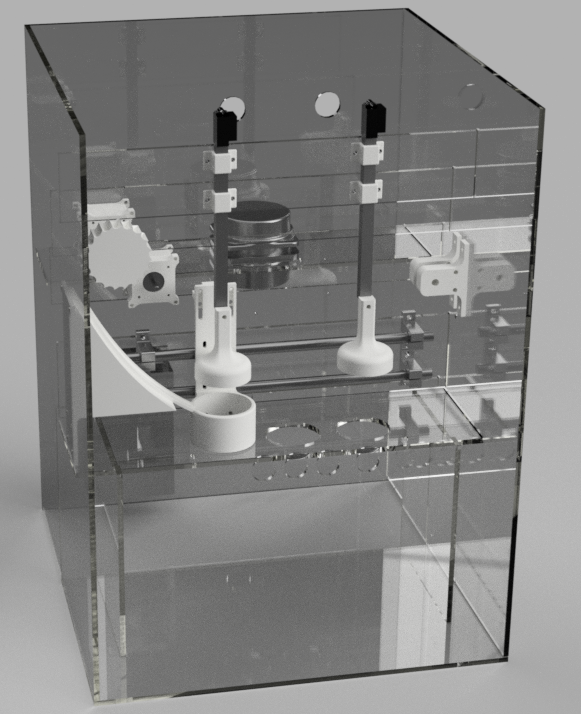
\includegraphics[width=1.8\columnwidth]{render}
    \caption{A render of the phyical system design.}
\end{figure*}

\subsection{Electronics and Control}
The electronics for the system were initially designed as
a custom PCB that would be responsible for all low-level
control tasks. This PCB would communicate over UART with
a Raspberry Pi 3 for WiFi control.

Due to outstanding issues with the motor control circuitry,
the system was redesigned to replace the custom PCB with an
Adafruit Feather board along with accessories that provided
equivalent functionality to what the original PCB was designed
for. In many cases, these accessories use components identical
to those used in the original PCB.

The electrical system consists for the following major
blocks: stepper motor controllers, PWM servo controllers, a
temperature sensor, relays, a liquid flow meter, and several
homing switches.

The stepper motor controller is an Adafruit Motor Controller
Featherwing. This controller uses a TB6613 H-bridge chip
along with the Arduino stepper motor library to control
the stepper. We additionally added a library (AccelStepper)
between the stepper motor library and the control chip for
moving the stepper motor with acceleration and deceleration.
We needed acceleration on the stepper movements for the puck
in order to achieve an accurate positioning.

Mechanisms involving stepper motors generally have a
certain point that is considered to be a starting, or home,
position. However, the starting position of the mechanism
may not necessarily be known. Therefore, the mechanism
must be �homed,� that is, the starting position must be found.
We accomplish this task in the tamp/brew/dispose mechanism
using two microswitches on either end of the device. On
startup, the puck is moved slowly to the tamper side of the
device until it runs into one of these homing switches. This
position is noted and the motor moves to the disposer side of
the machine until a switch on that end is hit, this position is
also noted. It�s important that we have accurate positions on
both ends of the mechanism in order to ensure that the tamper
and disposer are accurately positioned above the puck.

The temperature sensor is used to regulate the water temperature
in the boiler during the brewing process. The sensor
consists of thermocouple with an AD8494 temperature sensing
amplifer. A thermocouple is a device that produces a small
voltage depending on the temperature it is exposed to. This
voltage is too small for most microcontrollers to detect, so
it must be amplified. The AD8494 takes the thermocouple
voltage and amplifies it such that the output of the device is
5mV per degree Celsius.

A liquid flow meter was used to monitor the amount of fluid
being moved through the pump. This sensor has a pinwheel
with a magnet and a hall effect sensor. As fluid flow through
the sensor the pinwheel spins, causing the magnet to move
over the hall effect sensor, generating a digital pulse. Each
pulse equates to roughly 2.2mL of fluid. This signal was setup
to trigger an interrupt in the microcontroller. Each time this
interrupt is generated, a counter keeping track of how much
fluid has been dispensed is incremented.

When the system is started, the machine runs through a
startup check in which all motors and actuators are twitched
in order to verify correct functionality. The homing procedure
defined above is then performed. The machine will then move
the puck back to the tamping position and wait until a brew
command is received over UART. When this command is
received, the machine drives the motors and actuators to
perform the brewing process defined above. During the actual
brewing phase of the process, relays are used to turn on and
off the boiler and pump as described in the mechanical design
section. When the process is complete, the puck is returned to
the home position and the cycle repeats.

\begin{figure*}
  \centering
    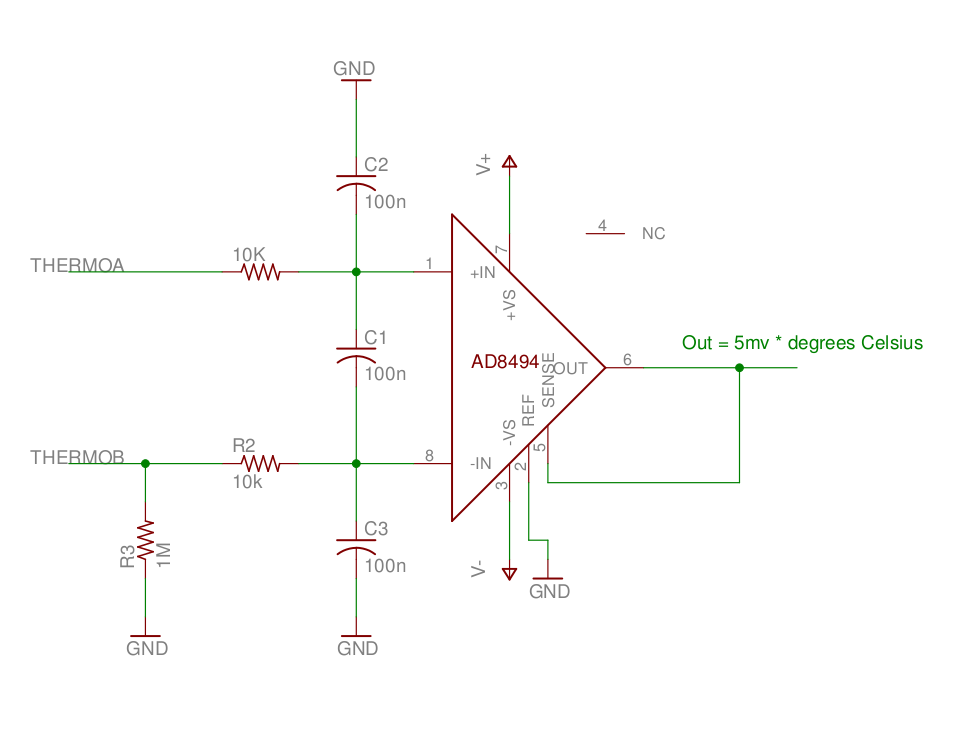
\includegraphics[width=1.8\columnwidth]{ThermoAmp}
    \caption{Thermocouple amplifier with 100Hz low-pass filter.}
\end{figure*}


% TODO This section should probably go after the flash section
\subsection{Raspberry Pi Setup and Initialization}
%TODO Actually build up and run http://mattrichardson.com/Raspberry-Pi-Flask/ on a flask server
% and right down the steps for setup. Setup should be very similar
 
%TODO This is written as if there will be microcontroller in conjunction with
% the RPI. I don't think that will wind up being the case - Aaron
% ADDENDUM I'm starting to think maybe that's not such a bad idea - Aaron
% ADDENDUM ADDENDUM We're using a seprate micro with the Pi.. - Aaron
\subsection{Flask}
Flask is a web framework that provides tools to allow you to build a web application.
Flask is a micro-framework, so it requires no outside dependencies or external libraries.
This means that Flask is lightweight. Flask is designed for creating web applications,
with a database backend that operates through the browser. We will be using it to open
a port on the local WiFi network that will act as a REST server. We will use
this server to send commands through the Raspberry Pi to the microcontroller. Thus, Flask is a middleman from the 
android application and the components inside the coffee machine.

\subsection{Mobile Application}
The UI was implemented on an Amazon Fire 7 tablet
running a Lollipop Android version application written in Java.
Upon opening the application, it will try to reconnect to the
previous device it was connected to and login the previously
logged in user, if either fields have been entered in the pase. If
it successfully connects to the last known device, it will take
them straight to main user control screen. If the tablet could
not connect to the device, the user has the option to start the
connection process, or decide to change the active profile.

Connecting to a device is simple. A screen for connecting
to a machine opens up, it shows a list of all of the coffee
machines that support the application in a recycler view. Once
one is selected, the user may try to connect. If the device
had previously connected properly then it will not prompt the
user for a password and attempt connection, otherwise the
user must input a password that is associated with the device
first. Ideally if this were a device being sold on a larger scale,
these passwords would be unique and sent out with the device
(perhaps a serial number would be used). Once the device is
connected it will move to the brewing functionality page. The
connection page also contains the functionality to change the
active user, scan the area for more machines, and return to the
main screen.

The brewing page has both basic and advanced options.
The basic options are the default active options and have just
a few settings for brewing the coffee: choosing how much,
how strong, and how frothy. The advanced settings have much
more to offer; selecting pressure, amount, and temperature for
milk, water, froth, syrup, and coffee. Not all of those will havethe same
available selections to change, but there is much higher customization in
advanced. We may be scrapping the ability to control pressure, but temperature
and amount are staying. From the brewing page we are also allowed to change
active users. With a user actively logged in, the option to use
the favourites feature comes into play for advanced settings.
This allows the user to load or delete favourites they have
previously saved and also save new ones. Once all settings
are where the user would like them, the brew button may be
pressed and the process shall be sent to the device. If the app
recognizes that it is a brew that was not loaded from favourites
and a user is logged in, it will ask the user if they would like
to save it as one and leave a description.

An extra feature was added to offer the user the option to
keep user data when clearing cache or data from application
settings in the Android settings. Since this information is not
remote, losing user data means it is lost forever, that is why
this feature was added.

\subsection{Communication between FLASK and App}
The Raspberry PI hosts it�s own web server that the
user communicates with. It has a REST API that will
allow us to control the board, and in turn the machine
as well. Within the android application itself, we use
Java.net. Within that class we are able to use things such
as HttpURLConnection to send HTTP requests such as
GET and POST requests. For Java HTTP GET requests we
can get all the info we need in a browser URL. We can
use static functions or functions with parameters within that
URL. An example of a GET request would be something like: \\ \\
\textbf{http://localhost:8080/CoffeeMaker/login?userName=Jim}\\ \\which could
be a request for the user information on a user named "Jim". We could also send
out information in a POST request that would be received on the local server
and then interpret the information and perform an action. There are also other
actions that are useful in REST API's such as PUT, PATCH, and DELETE. Steps
below are ones that would be used to send HTTP requests to the server using the
HttpURLConnection class:
\begin{itemize}
\item Create a URL object with a GET/POST URL string like one mentioned above
\item Open a connection with that URL that creates an instance of an HttpURLConnection
\item Set the request method in the HttpURLConnection
\item Call setRequestProperty() on HttpURLConnection
\item Call getResponseCode() to see if the request was processed successfully or
if there were errors
\item For GET, use a Reader and InputStream and process the response
\item For POST, before reading the response, get an OutputStream from
HttpURLConnection and write POST parameters into it.
\end{itemize} 
\ \\

\indent\textbf{The Flask API exposed calls} \\ 
\begin{itemize}
\item The first API call will be to verify that it is connected, this call will
be a GET call to verify connectivity. If the call succeeds a 200 response will
be posted as well as the session number, UTC timestamp, and model of the
machine in a json formatted payload.

\item The second API call will be to initiate a brewing cycle. 
This will be a POST call with machine settings embedded in the url or in a payload sent. If the
call succeeds a 201 response will be posted as well as session number, utc
timestamp, model and the data that was interpreted. If the machine is currently
making a cup of coffee, it will respond with a 200 response that indicates that
the machine is busy and the order will either be queued or discarded.
\end{itemize}

The REST API will be exposed to anyone on the network as it will run on host
'0.0.0.0'. '0.0.0.0' is a non-routable address that allows all IPV4 addresses
on the network to be listened to on the Raspberry Pi operating system.
However, each request will not be accepted by the machine unless it has a
serialized key that matches the machine data. Each machine will come with a
unique serial number that must be included in each request in order for the
request to be accepted. This will validate that a request is intentional and
legitimate.
The flask application will control and log every request made, as well as push
every coffee call up to an external database, making it the only device that is
pushing up to the database.

 In the case that we cannot complete the project the database element will be
scratched. This would affect the Flask part of the project such that the
expectation of data pushing and pulling will not be implemented.
If time does not permit us to complete the database section in whole, then the database loses all 
of its importance to this project and thus should not be attempted.

In the case that we cannot demonstrate our project at the University of Utah due to network protections,
we would buy / bring a popup wifi-network that we could connect to.

\subsubsection{UI Skeleton}

The mobile application consists of 6 activities,
2 fragments, a connection state machine, some data
classes, adapters, and customized widgets, etc. Quite a few
animations, layouts, and drawables were used in the application,
with the help of some 3rd party libraries as well. All
device info is saved in EXTERNAL STORAGE and all user
information is stored in Shared Preferences.

Most of the application is controlled by the WifiRunner
which has these main states: CONNECTED, WAITING
FOR USER, SEARCHING, CONNECT TO LAST,
WAITING FOR RESPONSE, NO WIFI, UNKNOWN. Each
activity behaves differently depending on the state of the this
thread. It also houses alot of the data communication for the
entire application. Any time a user does something, it sends
the WifiRunner into a different state and updates the current
activity with its results. When connected to a device, the
WifiRunner sends out a connection check requests to the flask
server on the RaspberryPi every second.

The MainMenu activity (shown in top half of Fig. 2)
consists of a two buttons, an animated background, and some
custom imageViews for backgrounds, logos, and buttons. A
3rd party library was used for a loading progress bar called
NewtonCradleLoading. This is used while trying to connect
to the previous device on this page. The �Connect Device�
button on this page allows the user to continue to the DeviceSelectioon
activity. The Login button opens a fragment
(shown in the bottom half of Fig. 2) to login a user or
opens dialogs, depending on the current active user state, and
updates to the label to the current user when when is logged
in. There is a logo in the top right labeled Beanster for the
application and there is also a wifi indicator in the top left that
displays whether or not the application is already successfully
connected to a coffee machine currently. When the application
starts, the WifiRunner tries to CONNECT TO LAST and
disables everything until it confirms whether or not it has
CONNECTED to the previous device or not. If it goes into a
CONNECTED state it kicks the application into the brewing
activity, otherwise it enables all of the buttons and displays a
disconnected symbol and is WAITING FOR USER.

The DeviceSelection activity (shown in Fig. 3) uses most
of the same components of the first activity, but introduces a
recyclerView and a couple other buttons as well. The recycler
view is populated by information from the WifiRunner. The
WifiRunner scans the network and looks for devices compatible
with the application and then sends all of the information
to the activity when it opens. The search button within this
activity allows the user to refresh that information inside
of the recyclerview. The back button returns to MainMenu
activity and the connect button sets the WifiRunner into
WAITING FOR RESPONSE to try and communicate with
the flask server hosted on the Raspberry PI. Depending on
the information on the device trying to be connected to, a
dialog might popup, prompting the user for a password for
the device. Depending on the response from the WifiRunner,
the activity warns that it couldn�t connect or continues to the
brewing activity.

The CoffeeBrew activity (shown in top half of Fig. 4) uses
a lot of the same widgets but a lot more of them. The new
features in this activity is the use of a customized slider and
spinner, but other than that, it is fairly simple. This page
keeps all info internally as it keeps track of the RequestData
information to be sent via http POST to the RaspberryPI. The
top two buttons change the rest of the center screen and give
different options. In the Basic State, a layout of 3 rows of
buttons appears that are given specific values for RequestData
and are set when pressed. When Advanced is clicked, more
tab options open with sliders available for each tab. These
are used to more finely adjust the RequestData before the
POST request. If a user is logged in and the Advanced button
is pressed, a favourites button is available, which opens a
Favourites fragment (shown in bottom of Fig. 4), allowing
loading and deletion of RequestData saves with labels that
are shown in a recycler view like the one previously in the
DeviceSelection activity.


\begin{figure}
    \begin{subfigure}
        \includegraphics[width=1\columnwidth]{mainmenu}
    \end{subfigure}
\hspace{5mm}
    \begin{subfigure}
	\frame{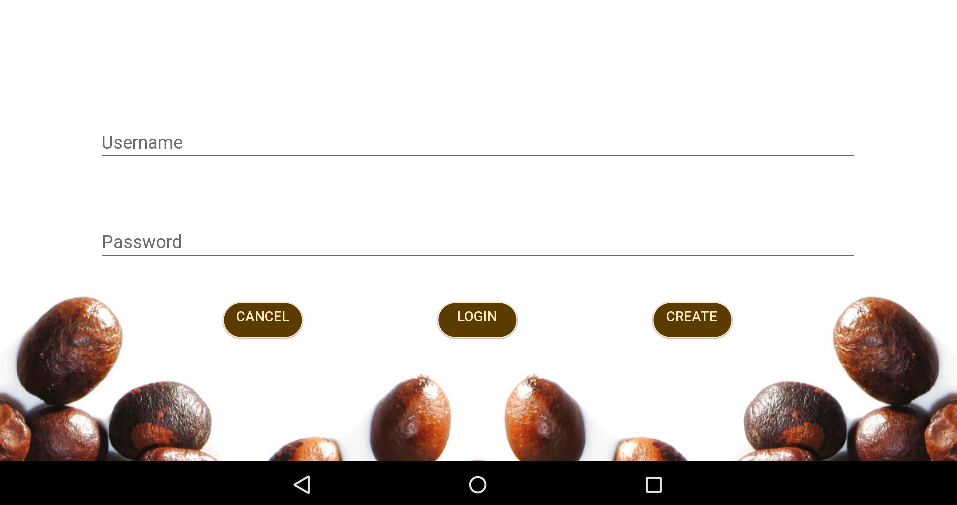
\includegraphics[width=1\columnwidth]{login}}
    \end{subfigure}
\caption{Opening screen for application and login fragment}
\end{figure}

In the brewing activity there will be many different widgets that control options
on the coffee machine. There are Spinners, Buttons, Sliders, Seekbars, etc. to control
the different mechanisms within the coffee machine. The different
mechanisms that will need control are temperatures of water/milk, PSI values for water/frothing,
amount of milk(ounces), amount of froth(percentage), what kind of syrup and how much, the amount of coffee, and the fineness
of coffee grounds. These will all be represented as integer values. Below is a mockup of the brewing activity:

\begin{figure}
\begin{subfigure}
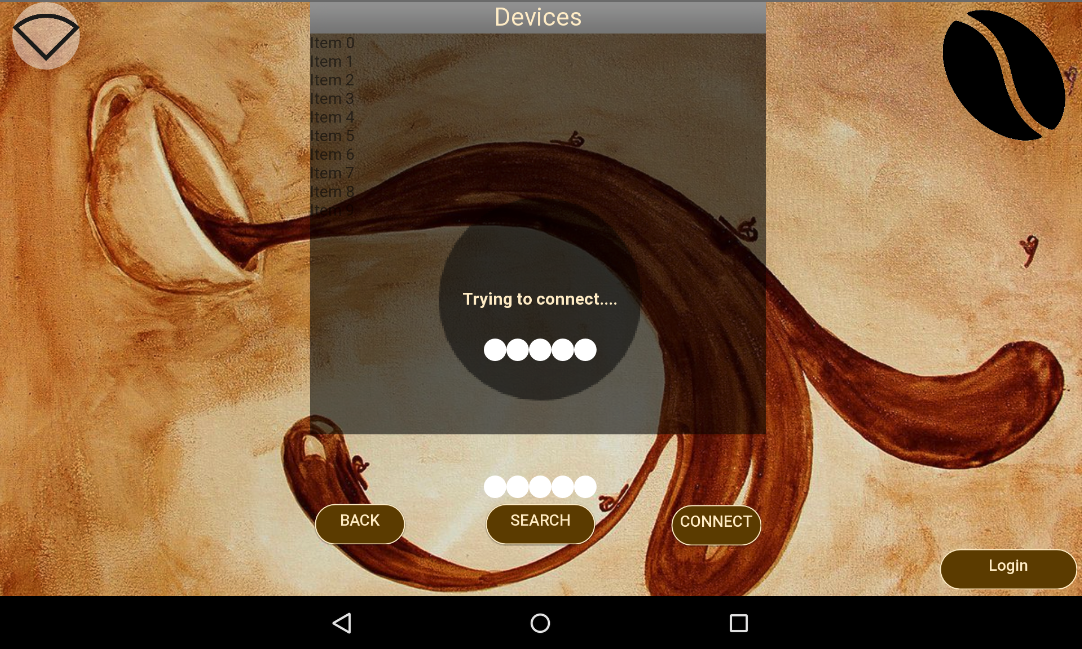
\includegraphics[width=1\columnwidth]{deviceSelection}
\end{subfigure}
\caption{Device selection page}
\end{figure} 

\begin{figure}
    \begin{subfigure}
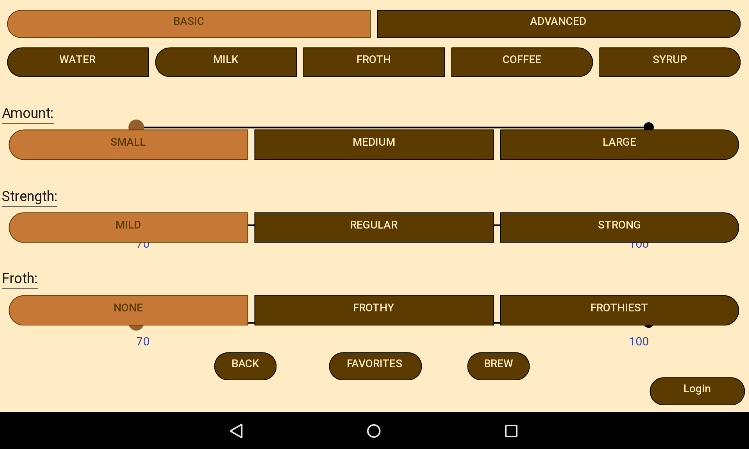
\includegraphics[width=1\columnwidth]{brew}
    \end{subfigure}
\hspace{5mm}
    \begin{subfigure}
\frame{\includegraphics[width=1\columnwidth]{favorites}}
    \end{subfigure}
\caption{Opening screen for application and login fragment}
\end{figure}

%\subsection{Data Aggregation and Processing Overview}
% The application will store user registrations, favorites, and other data in a standard SQL database. This database may be hosted separately from the machine, and could potentially be on a cloud service provider. The server will be encapsulated in an application server. The application server provides a container that can manage the database and its communication with the user application. The REST protocol will be used to communicate with the application server. Code running inside the application server will translate JSON or XML objects sent by the user into Java objects. Mappers will be used to dynamically translate these objects into SQL statements to update the database. The database will posses a users, beverages, and favorite's table. The users table will store core user data: name, email, salted password hashes, etc. The beverages table will store all of the settings you would need to instruct the coffee maker to produce an exact drink. Each beverage and user table row has a unique UUID. Each favorites list row will be connected to a single user via the UUID. Finally, each row of the favorites list will store all of the UUIDs that are associated with that list. That way, when a user sends a REST protocol request to get all of the favorites list of a particular user, the mapper can generate a SELECT request to grab all the relevant lists from the favorites table and then use the uuids stored within those rows of the favorites table to grab the drinks associated with each list. All the aggregated data is then returned to the user via REST protocol. 
%The application will store machine data, and individual coffee customizations in a standard SQL database. 
%The database will be hosted on a cloud service provider (AmazonS3 or Firebase). Each machine will have it's own table for statistics on its own components to document wear and usage. 
%Coffee customizations will be in a global database table where it will store information about the individual customizations of the cup of coffee as well as the serialized number for the coffee machine, for
%ease in sorting through machine by machine usage.

% Include a discussion of how well the device works here
\section{Evaluation}
When we started this project we set out to make a perfect coffee machine that
could do it all. Brew, froth, grind, dispense, and even more. We quickly found,
however, that creating just an automatic tamper/brewer was months of work
in and of itself. We had to start scaling back our expectations pretty
quickly into the project. There were also some unexpected pitfalls throughout
the course of the project. Our custom PCB not working as expected set us back by
two weeks, at least. We had to scramble fast to come up with an alternate
solution.

Ultimately however, the result of our work is pretty functional and something
that we can really be proud of. We successfully designed and implemented a
frightenly complex machine with a complicated embedded system and an Android app, and it
all works toghether to actually make espresso, just like we wanted.

The tamping and brewing mechanism worked as designed after only two iterations
of the 3D printed parts. We sucessfully wrote code to acuratly move and home
stepper motors, and the machine continues to maintain its accuracy after
repeated runs. That is, the machine doesn't get knocked out of alignement after
a use or two. It will function indefinetly.

Comparing our machine to existing automatic espresso machines, our
implementation falls a little flat in comparision due to the complexity and
costs invloved with our machine. A standard home automatic espresso machine
costs somewhere between \$1000 and \$2000. If our machine were to be produced
and sold as is, it would likely cost twice that amount. Although we set out with a
final product in mind, this machine is a proof of concept. Additional work by a
balanced engineering team with substantial funding would be needed to take the
machine to a point where it could be a competive product. 

Our machine does, however, demonstrate that the espresso making process can be
automated in a way that mimics the way in which a human would manually produce
espresso.
% Include a section solely for Demo Day Evaluation
\subsection{Demo Day Evaluation}
% Each do a an individual evaluation, then stitch together
% Ben
% 
% XXX - Uncomment before next push
% The demo day presentation seemed to impress a lot of people. While we didn't 
% have a functioning machine due to blowing out our pump on the day before, 
% we still had a very precise and elegant machine. We were able to demo a 'dry-run' 
% of exactly what would be happening throughout the entire process. 
% This 'dry-run' showed off the multiple different application of motors and actuators used in our project.
% I think people understood and appreciated the effort that was put into the precise machining and operation 
% of our project even if it was not complete. People also seemed to appreciate the fluidity and ease of the 
% mobile application which is a credit to Nathan and his hard work.
% 

The night before demo day, the pump being used to push water through the boiler
failed (the exact cause of the failure is unknown, but it's likely due to
overuse). Because of this, we were not able to do produce espresso with the
machine. We were, however, able to effectively demonstrate all of the novel
mechanisms, hardware, and software that were developed for the machine. We did
this by doing dry runs of the machine in which all of the steps for making
espresso described above were performed when evoked by our Android application.

Those viewing the demonstration seemed to be impressed with the machine, and we
got several compliments for sucessfully putting together all of the mechanisms
and for the fluidity with which the whole setup ran.

The feedback we received on demo day validated the project and the months of
hard work we put into our machine.

\section{Appendix A: Discoveries and Pitfalls}
% Never open a project by designing a PCB
\subsection{Never Start with a PCB}
When we first started the project, the very first thing we did was design a
large, complicated PCB that had all of the circuitry that we \italics{thought}
we would need.

After we got the PCB back and assembled it we discovered that while the
majority of the board functioned as expected, our motor controller circuitry did
not function. 

Designing and building this board was about a month long process, and that time
was largely wasted. After a few nights of frantically and pointlessly trying to
get the board to work, we decided it would be better to switch over to using
off the shelf Arduino boards and accessories.

Had we started with the Arduino setup, we would have had substantially more time
to iron out any issues with the mechanical side of the project. If there was
time, we could have then based a PCB on our prototype setup, which would have
been much more likely to work as expected.

% If there's a mechanical aspect to the problem, always start with the
% mechanical aspect

% Be weary of heavy inductive loads
\subsection{Inductive Loads}
We drove our vibratory espresso pump via a relay connected to 120V mains.
Ocassionally when we opened up the relay driving the pump, the machine reset.
The pump and the digital side of the system were electrically isolated, but were
in a fairly close physical proximity and some digital control lines ran fairly
close to the pump.

It turns out that when the pump was being disconnected from power, the leftover
energy stored in the pump's coil caused a large voltage spike across the pump
terminals. The spike was sufficent to create a large burst of electromagnetic
interference that induced a voltage on the digital side of the system that was
sufficent to cause a reset in the control board.

To solve this issue, we placed a large 2mF capacitor with a bleeder resistor
across the pump terminals in order to supress the inductive spiking.


% Have a spare of everything
\subsection{Have a Spare of Everything}
We went through the whole project having, for the most part, exact quantities of
the components we needed. For most of the project this wasn't an issue. When our
only brewing pump failed the night before demo day however, it became clear that
we should have been keeping spares around. 

We salvaged our pump from a consumer Delonghi espresso machine that we picked
up in a ``for parts'' state on Ebay. The type of vibratory pump that we were
using is known for its short lifespan and in hindsight, we should have thought
to find another one. 

It turns out we could have picked up an idential, never used, pump online for
\$50, a price that would have been well worth saving our demo.

\section{Appendix B: Code Archive}
\begin{itemize}
\item Embedded Code - \href{https://github.com/pabstaaron/AutoCoffeeMaker/tree/master/Arduino\%20Code}
\item Android Code - \href{https://github.com/pabstaaron/AutoCoffeeMaker/tree/master/Beanster}
\item Web Page Code - \href{https://github.com/pabstaaron/AutoCoffeeMaker/tree/master/docs}
\item Flask Code - \href{https://github.com/pabstaaron/AutoCoffeeMaker/tree/master/flask\_server}
\end{itemize}


\section{Appendix B: Bill of Materials}
\begin{itemize}
\item Raspberry Pi 3
\item Espresso Boiler 
\item Vibratory Pump
\item Adafruit Feather
\item Adafruit Motor Control
\item Copper pipe
\item Silicone Tubing
\item PETG Filament
\item Stepper motors
\item Peristaltic pumps
\item Thermocouples
\item AD8494 Thermocouple Amplifiers
\item Acrylic
\item NEMA-17 Stepper Motors
\item 12mm Steel Rod
\item 12mm Pillow Block
\item Bearings
\item 12mm Rail Mounts
\item Flow Meter
\end{itemize}

\bibliography{biblio}{}
\bibliographystyle{plain}

\end{document}
\end
